% answers.tex —— 2012 年·江苏卷 · 参考答案与详细解析片段
% 由 tools/generate_projects.py 依来源总账自 2012/2012_数学真题_江苏_试题.md + 2012/2012_数学真题_江苏_解析正文.md + 2012/2012_数学真题_江苏_答案要点.md 生成，勿手改（改源 MD 后重跑）


\begin{answer}
\gksolhead{1}{}

\textbf{题目}：

已知集合 $A=\{1,2,4\}$，$B=\{2,4,6\}$，则 $A\cup B=$ $\underline{\qquad}$。

\Needspace{4\baselineskip}
\textbf{解析}

\Needspace{5\baselineskip}
$A$ 中元素为 $1,2,4$，$B$ 中元素为 $2,4,6$。并集要求把两个集合的元素全部列出，公共元素只写一次，因此
\nopagebreak[4]
\[A\cup B=\{1,2,4,6\}.\]
$A\cup B$ 含 $4$ 个元素，不少于 $A$、$B$ 中任一集合的元素个数，符合并集的基本性质。

\gkanswer{答案：$\{1,2,4,6\}$。两集合的公共元素只写一次，$A$ 的元素与 $B$ 的元素合并即得。}

\end{answer}
\begin{answer}
\gksolhead{2}{}

\textbf{题目}：

某学校高一、高二、高三年级的学生人数之比是 $3:3:4$，现用分层抽样的方法从该校高中三个年级的学生中抽取容量为 $50$ 的样本，则应从高二年级抽取 $\underline{\qquad}$ 名学生。

\Needspace{4\baselineskip}
\textbf{解析}

\Needspace{5\baselineskip}
分层抽样按各层人数比例分配样本容量。三个年级人数比为
\nopagebreak[4]
\[3:3:4,\]
\Needspace{5\baselineskip}
总份数为 $3+3+4=10$，故每份对应
\nopagebreak[4]
\[\frac{50}{10}=5\text{ \text{人}}.\]
\Needspace{5\baselineskip}
高二年级占 $3$ 份，应抽取
\nopagebreak[4]
\[3\times5=15\text{ \text{人}}.\]
核对：高一、高二、高三分别抽取 $15,15,20$ 人，合计 $50$ 人，与样本容量一致。

\gkanswer{答案：$15$。高二年级占 $3:3:4$ 中的 $3$ 份，按比例抽取 $50\times\dfrac3{10}=15$ 名。}

\end{answer}
\begin{answer}
\gksolhead{3}{}

\textbf{题目}：

设 $a$，$b\in\mathbf R$，$a+b\mathrm i=\dfrac{11-7\mathrm i}{1-2\mathrm i}$（$\mathrm i$ 为虚数单位），则 $a+b$ 的值为 $\underline{\qquad}$。

\Needspace{4\baselineskip}
\textbf{解析}

\Needspace{5\baselineskip}
分母实数化，分子分母同乘 $1+2\mathrm i$：
\nopagebreak[4]
\[\frac{11-7\mathrm i}{1-2\mathrm i}=\frac{(11-7\mathrm i)(1+2\mathrm i)}{(1-2\mathrm i)(1+2\mathrm i)}.\]
\Needspace{5\baselineskip}
分子展开
\nopagebreak[4]
\[(11-7\mathrm i)(1+2\mathrm i)=11+22\mathrm i-7\mathrm i-14\mathrm i^2=25+15\mathrm i,\]
\Needspace{5\baselineskip}
分母为 $1^2+2^2=5$，故
\nopagebreak[4]
\[a+b\mathrm i=\frac{25+15\mathrm i}{5}=5+3\mathrm i.\]
\Needspace{5\baselineskip}
由复数相等的定义得 $a=5$，$b=3$，所以
\nopagebreak[4]
\[a+b=8.\]

\gkanswer{答案：$8$。分母实数化得 $a+b\mathrm i=5+3\mathrm i$，故 $a=5$，$b=3$。}

\end{answer}
\begin{answer}
\gksolhead{4}{}

\textbf{题目}：

如图是一个算法流程图，则输出的 $k$ 的值是 $\underline{\qquad}$。
\nopagebreak[4]
\begin{center}% ============================================================
% f2012_jiangsu_q04_flowchart.tex
% 2012 江苏卷第 4 题 算法流程图（TikZ 矢量重绘）
% 开始 → k←1 → 判断 k^2-5k+4>0；否：k←k+1 回代；是：输出 k → 结束
% ============================================================
\begin{tikzpicture}[
  x=1cm, y=1cm, line width=0.6pt, font=\footnotesize, >=Stealth,
  every node/.style={inner sep=3pt},
  proc/.style={rectangle, draw, minimum width=2.4cm, minimum height=0.62cm},
  io/.style={trapezium, draw, trapezium left angle=70, trapezium right angle=110,
             minimum width=2.8cm, minimum height=0.66cm},
  dec/.style={diamond, draw, aspect=2.6, minimum width=3.4cm, minimum height=0.95cm},
  term/.style={rectangle, rounded corners=8pt, draw, minimum width=2.0cm,
               minimum height=0.58cm}
]

  \node[term] (start) at (0,0) {开始};
  \node[proc] (init)  at (0,-1.35) {$k\leftarrow1$};
  \node[dec]  (judge) at (0,-2.95) {$k^2-5k+4>0$};
  \node[proc] (inc)   at (4.10,-2.95) {$k\leftarrow k+1$};
  \node[io]   (out)   at (0,-4.45) {输出 $k$};
  \node[term] (end)   at (0,-5.75) {结束};

  \draw[->] (start) -- (init);
  \draw[->] (init) -- (judge);
  \draw[->] (judge) -- (out);
  \node at (0.55,-3.62) {Y};
  \draw[->] (out) -- (end);
  \draw[->] (judge.east) -- node[above] {N} (inc.west);

  % 否：k←k+1 之后回到判断框之前
  \draw[->] (inc.north) -- (4.10,-1.95) -- (0,-1.95);

\end{tikzpicture}
\end{center}
\nopagebreak[4]
\Needspace{4\baselineskip}
\textbf{解析}

按框图顺序执行，循环体只有 $k\leftarrow k+1$，判断条件为 $k^2-5k+4>0$。

\begin{itemize}
\item $k=1$：$1-5+4=0$，不满足，$k$ 变为 $2$；
\item $k=2$：$4-10+4=-2$，不满足，$k$ 变为 $3$；
\item $k=3$：$9-15+4=-2$，不满足，$k$ 变为 $4$；
\item $k=4$：$16-20+4=0$，不满足，$k$ 变为 $5$；
\item $k=5$：$25-25+4=4>0$，满足，输出 $k=5$。
\end{itemize}

所以输出的 $k$ 的值是 $5$。

（说明：$k^2-5k+4=(k-1)(k-4)$，故 $k=1,4$ 时取零、$k=2,3$ 时取负值，前四次判断均不成立。）

\gkanswer{答案：$5$。依次检验 $k=1,2,3,4$ 均不满足 $k^2-5k+4>0$，$k=5$ 时 $5^2-25+4=4>0$，输出 $5$。}

\end{answer}
\begin{answer}
\gksolhead{5}{}

\textbf{题目}：

函数 $f(x)=\sqrt{1-2\log_6x}$ 的定义域为 $\underline{\qquad}$。

\Needspace{4\baselineskip}
\textbf{解析}

\Needspace{5\baselineskip}
要使 $f(x)=\sqrt{1-2\log_6x}$ 有意义，需被开方式非负：
\nopagebreak[4]
\[1-2\log_6x\geqslant0\Longrightarrow\log_6x\leqslant\frac12.\]
\Needspace{5\baselineskip}
因为底数 $6>1$，对数函数单调递增，故
\nopagebreak[4]
\[0<x\leqslant6^{\frac12}=\sqrt6,\]
\Needspace{5\baselineskip}
其中 $x>0$ 来自对数的定义域。所以定义域为
\nopagebreak[4]
\[\left(0,\sqrt6\right].\]
核对：$x=\sqrt6$ 时 $\log_6x=\dfrac12$，被开方式为 $0$，可以取到；$x\to0^{+}$ 时 $\log_6x\to-\infty$，被开方式为正，故左端开。

\gkanswer{答案：$(0,\sqrt6]$。被开方式非负给出 $\log_6x\leqslant\dfrac12$，再与对数定义域 $x>0$ 取交。}

\end{answer}
\begin{answer}
\gksolhead{6}{}

\textbf{题目}：

现有 $10$ 个数，它们能构成一个以 $1$ 为首项，$-3$ 为公比的等比数列，若从这 $10$ 个数中随机抽取一个数，则它小于 $8$ 的概率是 $\underline{\qquad}$。

\Needspace{4\baselineskip}
\textbf{解析}

\Needspace{5\baselineskip}
等比数列的首项 $a_1=1$，公比 $q=-3$，故这 $10$ 个数为
\nopagebreak[4]
\[a_k=(-3)^{k-1}\quad(k=1,2,\cdots,10),\]
\Needspace{5\baselineskip}
即
\nopagebreak[4]
\[1,\ -3,\ 9,\ -27,\ 81,\ -243,\ 729,\ -2187,\ 6561,\ -19683.\]
\Needspace{5\baselineskip}
逐一比较与 $8$ 的大小：$k$ 为偶数时 $a_k<0<8$，共 $5$ 个（$k=2,4,6,8,10$）；$k$ 为奇数时 $a_k=3^{k-1}>0$，只有 $k=1$ 时 $a_1=1<8$，$k=3,5,7,9$ 时 $a_k\geqslant9>8$。故小于 $8$ 的数共
\nopagebreak[4]
\[5+1=6\text{ \text{个}}.\]
\Needspace{5\baselineskip}
从 $10$ 个数中随机抽取一个，概率为
\nopagebreak[4]
\[P=\frac{6}{10}=\frac35.\]

\gkanswer{答案：$\dfrac35$。这 $10$ 个数为 $1,-3,9,\cdots,(-3)^9$，小于 $8$ 的为 $1$ 与 $5$ 个负数，共 $6$ 个。}

\end{answer}
\begin{answer}
\gksolhead{7}{}

\textbf{题目}：

如图，在长方体 $ABCD-A_1B_1C_1D_1$ 中，$AB=AD=3$ cm，$AA_1=2$ cm，则四棱锥 $A-BB_1D_1D$ 的体积为 $\underline{\qquad}$ cm$^3$。
\nopagebreak[4]
\begin{center}% ============================================================
% f2012_jiangsu_q07_cuboid.tex
% 2012 江苏卷第 7 题 长方体 ABCD-A1B1C1D1 与四棱锥 A-BB1D1D
% AB=AD=3 cm，AA1=2 cm（TikZ 矢量重绘）
% ============================================================
\begin{tikzpicture}[x=1cm, y=1cm, line width=0.6pt, font=\footnotesize]

  \coordinate (A)  at (0,0);
  \coordinate (B)  at (3.0,0);
  \coordinate (C)  at (4.2,1.15);
  \coordinate (D)  at (1.2,1.15);
  \coordinate (A1) at (0,1.85);
  \coordinate (B1) at (3.0,1.85);
  \coordinate (C1) at (4.2,3.00);
  \coordinate (D1) at (1.2,3.00);

  % ---------- 长方体的棱 ----------
  \draw (A) -- (B) -- (C);
  \draw[dashed] (C) -- (D) -- (A);
  \draw (A) -- (A1);
  \draw (B) -- (B1);
  \draw (C) -- (C1);
  \draw[dashed] (D) -- (D1);
  \draw (A1) -- (B1) -- (C1) -- (D1) -- cycle;

  % ---------- 四棱锥 A-BB1D1D ----------
  \draw (B) -- (B1);
  \draw (B1) -- (D1);
  \draw[dashed] (D1) -- (D);
  \draw[dashed] (D) -- (B);
  \draw (A) -- (B1);
  \draw[dashed] (A) -- (D1);

  % ---------- 标注 ----------
  \node[below left]  at (A)  {$A$};
  \node[below]       at (B)  {$B$};
  \node[right]       at (C)  {$C$};
  \node at ($(D)+(-0.34,0.24)$) {$D$};
  \node[left]        at (A1) {$A_1$};
  \node[right]       at (B1) {$B_1$};
  \node[above right] at (C1) {$C_1$};
  \node[above]       at (D1) {$D_1$};

\end{tikzpicture}
\end{center}
\nopagebreak[4]
\Needspace{4\baselineskip}
\textbf{解析}

\Needspace{5\baselineskip}
以 $A$ 为原点，$\overrightarrow{AB}$、$\overrightarrow{AD}$、$\overrightarrow{AA_1}$ 为坐标轴方向建立空间直角坐标系，则
\nopagebreak[4]
\[A(0,0,0),\ B(3,0,0),\ D(0,3,0),\ B_1(3,0,2),\ D_1(0,3,2).\]
\Needspace{5\baselineskip}
四棱锥 $A-BB_1D_1D$ 的底面是矩形 $BB_1D_1D$：$\overrightarrow{BB_1}=(0,0,2)$，$\overrightarrow{BD}=(-3,3,0)$，两者垂直，故
\nopagebreak[4]
\[S_{BB_1D_1D}=|BB_1|\cdot|BD|=2\times3\sqrt2=6\sqrt2.\]
\Needspace{5\baselineskip}
平面 $BB_1D_1D$ 过 $B(3,0,0)$、$D(0,3,0)$ 且平行于 $z$ 轴，其方程为 $x+y=3$。点 $A$ 到该平面的距离为
\nopagebreak[4]
\[h=\frac{|0+0-3|}{\sqrt{1^2+1^2}}=\frac{3}{\sqrt2}.\]
\Needspace{5\baselineskip}
所以体积
\nopagebreak[4]
\[V=\frac13 S_{BB_1D_1D}\cdot h=\frac13\times6\sqrt2\times\frac{3}{\sqrt2}=6\ \left(\text{cm}^3\right).\]
\Needspace{5\baselineskip}
核对：用混合积独立复算。底面 $BB_1D_1D$ 是平行四边形，四棱锥体积等于三棱锥 $A-BB_1D_1$ 体积的两倍：
\nopagebreak[4]
\[V=2\cdot\frac16\left|\begin{vmatrix}3&0&0\\3&0&2\\0&3&2\end{vmatrix}\right|=2\cdot\frac{18}{6}=6,\]
与上式一致（体积单位为 cm$^3$）。

\gkanswer{答案：$6$。底面 $BB_1D_1D$ 为矩形，面积 $6\sqrt2$，$A$ 到该平面的距离为 $\dfrac{3}{\sqrt2}$。}

\end{answer}
\begin{answer}
\gksolhead{8}{}

\textbf{题目}：

在平面直角坐标系 $xOy$ 中，若双曲线 $\dfrac{x^2}{m}-\dfrac{y^2}{m^2+4}=1$ 的离心率为 $\sqrt5$，则 $m$ 的值为 $\underline{\qquad}$。

\Needspace{4\baselineskip}
\textbf{解析}

\Needspace{5\baselineskip}
双曲线 $\dfrac{x^2}{m}-\dfrac{y^2}{m^2+4}=1$ 的实半轴平方 $a^2=m$，虚半轴平方 $b^2=m^2+4$，故
\nopagebreak[4]
\[e^2=1+\frac{b^2}{a^2}=1+\frac{m^2+4}{m}.\]
\Needspace{5\baselineskip}
由 $e=\sqrt5$ 得 $e^2=5$，即
\nopagebreak[4]
\[1+\frac{m^2+4}{m}=5\Longrightarrow\frac{m^2+4}{m}=4\Longrightarrow m^2-4m+4=0,\]
\Needspace{5\baselineskip}
所以
\nopagebreak[4]
\[(m-2)^2=0\Longrightarrow m=2.\]
核对：$m=2$ 时 $a^2=2$，$b^2=8$，$e^2=1+\dfrac82=5$，与题设一致；且 $m=2>0$ 使方程确为双曲线。

\gkanswer{答案：$2$。由 $e^2=1+\dfrac{m^2+4}{m}=5$ 得 $m^2-4m+4=0$，故 $m=2$。}

\end{answer}
\begin{answer}
\gksolhead{9}{}

\textbf{题目}：

如图，在矩形 $ABCD$ 中，$AB=\sqrt2$，$BC=2$，点 $E$ 为 $BC$ 的中点，点 $F$ 在边 $CD$ 上，若 $\overrightarrow{AB}\cdot\overrightarrow{AF}=\sqrt2$，则 $\overrightarrow{AE}\cdot\overrightarrow{BF}$ 的值是 $\underline{\qquad}$。
\nopagebreak[4]
\begin{center}% ============================================================
% f2012_jiangsu_q09_rectangle.tex
% 2012 江苏卷第 9 题 矩形 ABCD，E 为 BC 中点，F 在边 CD 上
% AB=√2，BC=2；图中标出向量 AB、AF、AE（TikZ 矢量重绘）
% ============================================================
\begin{tikzpicture}[x=1cm, y=1cm, line width=0.6pt, font=\footnotesize, >=Stealth]

  \coordinate (A) at (0,0);
  \coordinate (B) at (2.20,0);
  \coordinate (C) at (2.20,3.10);
  \coordinate (D) at (0,3.10);
  \coordinate (E) at (2.20,1.55);
  \coordinate (F) at (1.556,3.10);

  % ---------- 矩形 ----------
  \draw (A) -- (B) -- (C) -- (D) -- cycle;

  % ---------- 向量 ----------
  \draw[->] (A) -- (B);
  \draw[->] (A) -- (F);
  \draw[->] (A) -- (E);

  % ---------- 标注 ----------
  \node[below left]  at (A) {$A$};
  \node[below right] at (B) {$B$};
  \node[right]       at (C) {$C$};
  \node[left]        at (D) {$D$};
  \node[right]       at (E) {$E$};
  \node[above]       at (F) {$F$};

\end{tikzpicture}
\end{center}
\nopagebreak[4]
\Needspace{4\baselineskip}
\textbf{解析}

\Needspace{5\baselineskip}
以 $A$ 为原点、$\overrightarrow{AB}$ 为 $x$ 轴正方向建立直角坐标系，则
\nopagebreak[4]
\[A(0,0),\ B(\sqrt2,0),\ C(\sqrt2,2),\ D(0,2).\]
\Needspace{5\baselineskip}
$E$ 为 $BC$ 中点，故 $E\left(\sqrt2,1\right)$。设 $F(t,2)$（$0\leqslant t\leqslant\sqrt2$），则
\nopagebreak[4]
\[\overrightarrow{AB}=(\sqrt2,0),\qquad\overrightarrow{AF}=(t,2),\]
\Needspace{5\baselineskip}
由 $\overrightarrow{AB}\cdot\overrightarrow{AF}=\sqrt2$ 得
\nopagebreak[4]
\[\sqrt2\,t=\sqrt2\Longrightarrow t=1,\]
即 $F(1,2)$（确实在边 $CD$ 上）。

\Needspace{5\baselineskip}
于是
\nopagebreak[4]
\[\overrightarrow{AE}=\left(\sqrt2,1\right),\qquad\overrightarrow{BF}=\left(1-\sqrt2,2\right),\]
\nopagebreak[4]
\[\overrightarrow{AE}\cdot\overrightarrow{BF}=\sqrt2\left(1-\sqrt2\right)+1\times2=\sqrt2-2+2=\sqrt2.\]
所以 $\overrightarrow{AE}\cdot\overrightarrow{BF}=\sqrt2$。

\gkanswer{答案：$\sqrt2$。以 $A$ 为原点建系，由 $\overrightarrow{AB}\cdot\overrightarrow{AF}=\sqrt2$ 定出 $F(1,2)$，再算 $\overrightarrow{AE}\cdot\overrightarrow{BF}$。}

\end{answer}
\begin{answer}
\gksolhead{10}{}

\textbf{题目}：

\Needspace{5\baselineskip}
设 $f(x)$ 是定义在 $\mathbf R$ 上且周期为 $2$ 的函数，且在区间 $[-1,1]$ 上，
\nopagebreak[4]
\[f(x)=\begin{cases}ax+1,&-1\leqslant x<0,\\[2pt]\dfrac{bx+2}{x+1},&0\leqslant x\leqslant1,\end{cases}\]
其中 $a$，$b\in\mathbf R$。若 $f\left(\dfrac12\right)=f\left(\dfrac32\right)$，则 $a+3b$ 的值为 $\underline{\qquad}$。

\Needspace{4\baselineskip}
\textbf{解析}

\Needspace{5\baselineskip}
$f(x)$ 的周期为 $2$，故
\nopagebreak[4]
\[f\left(\frac32\right)=f\left(\frac32-2\right)=f\left(-\frac12\right),\qquad f(1)=f(-1).\]
在 $[-1,1]$ 上 $f(x)$ 由两段给出：$-1\leqslant x<0$ 时取 $ax+1$，$0\leqslant x\leqslant1$ 时取 $\dfrac{bx+2}{x+1}$。故 $f\left(\dfrac12\right)$、$f(1)$ 用第二段，$f\left(-\dfrac12\right)$、$f(-1)$ 用第一段。

\Needspace{5\baselineskip}
由周期得 $f\left(\dfrac12\right)=\dfrac{\dfrac b2+2}{\dfrac12+1}=\dfrac{b+4}{3}$，$f\left(-\dfrac12\right)=-\dfrac a2+1$，代入 $f\left(\dfrac12\right)=f\left(\dfrac32\right)$：
\nopagebreak[4]
\[\frac{b+4}{3}=1-\frac a2\Longrightarrow2b+8=6-3a\Longrightarrow3a+2b=-2. \tag{1}\]
\Needspace{5\baselineskip}
再由 $f(1)=f(-1)$：$f(1)=\dfrac{b+2}{2}$，$f(-1)=-a+1$，得
\nopagebreak[4]
\[\frac{b+2}{2}=1-a\Longrightarrow b+2=2-2a\Longrightarrow2a+b=0. \tag{2}\]
\Needspace{5\baselineskip}
由 $(2)$ 得 $b=-2a$，代入 $(1)$：
\nopagebreak[4]
\[3a-4a=-2\Longrightarrow a=2,\qquad b=-4.\]
\Needspace{5\baselineskip}
所以
\nopagebreak[4]
\[a+3b=2-12=-10.\]
核对：$a=2$，$b=-4$ 时 $f\left(\dfrac12\right)=\dfrac{0}{3}=0$，$f\left(\dfrac32\right)=f\left(-\dfrac12\right)=-1+1=0$，两端相等；$f(1)=-1=f(-1)$，均成立。

\gkanswer{答案：$-10$。由周期 $2$ 得 $f\left(\dfrac32\right)=f\left(-\dfrac12\right)$，与 $f(1)=f(-1)$ 联立解得 $a=2$，$b=-4$。}

\end{answer}
\begin{answer}
\gksolhead{11}{}

\textbf{题目}：

设 $\alpha$ 为锐角，若 $\cos\left(\alpha+\dfrac\pi6\right)=\dfrac45$，则 $\sin\left(2\alpha+\dfrac\pi{12}\right)$ 的值为 $\underline{\qquad}$。

\Needspace{4\baselineskip}
\textbf{解析}

\Needspace{5\baselineskip}
设 $\beta=\alpha+\dfrac\pi6$。由 $\cos\beta=\dfrac45$ 且 $\alpha$ 为锐角知 $\beta\in\left(\dfrac\pi6,\dfrac{2\pi}3\right)$，而 $\cos\beta>0$，故 $\beta\in\left(\dfrac\pi6,\dfrac\pi2\right)$，从而
\nopagebreak[4]
\[\sin\beta=\frac35.\]
\Needspace{5\baselineskip}
所求角可化为
\nopagebreak[4]
\[2\alpha+\frac\pi{12}=2\left(\beta-\frac\pi6\right)+\frac\pi{12}=2\beta-\frac\pi4.\]
\Needspace{5\baselineskip}
由二倍角公式
\nopagebreak[4]
\[\sin2\beta=2\sin\beta\cos\beta=\frac{24}{25},\qquad\cos2\beta=\cos^2\beta-\sin^2\beta=\frac{16-9}{25}=\frac7{25}.\]
\Needspace{5\baselineskip}
于是
\nopagebreak[4]
\[\sin\left(2\beta-\frac\pi4\right)=\sin2\beta\cos\frac\pi4-\cos2\beta\sin\frac\pi4=\frac{\sqrt2}{2}\left(\frac{24}{25}-\frac7{25}\right)=\frac{17\sqrt2}{50}.\]
数值核对：$\beta\approx36.87^\circ$，$2\beta-45^\circ\approx28.74^\circ$，$\sin28.74^\circ\approx0.481$，与 $\dfrac{17\sqrt2}{50}\approx0.481$ 一致；结果在 $(0,1)$ 内，合理。

\gkanswer{答案：$\dfrac{17\sqrt2}{50}$。令 $\beta=\alpha+\dfrac\pi6$，则所求为 $\sin\left(2\beta-\dfrac\pi4\right)$，用二倍角与差角公式。}

\end{answer}
\begin{answer}
\gksolhead{12}{}

\textbf{题目}：

在平面直角坐标系 $xOy$ 中，圆 $C$ 的方程为 $x^2+y^2-8x+15=0$，若直线 $y=kx-2$ 上至少存在一点，使得以该点为圆心，$1$ 为半径的圆与圆 $C$ 有公共点，则 $k$ 的最大值是 $\underline{\qquad}$。

\Needspace{4\baselineskip}
\textbf{解析}

\Needspace{5\baselineskip}
圆 $C$ 的方程配方：
\nopagebreak[4]
\[x^2-8x+16+y^2=1\Longrightarrow(x-4)^2+y^2=1,\]
圆心 $C(4,0)$，半径 $1$。

题设“以直线上某点为圆心、$1$ 为半径的圆与圆 $C$ 有公共点”等价于：存在直线 $y=kx-2$ 上的点，它到 $C$ 的距离不超过 $1+1=2$（两圆半径之和）。

\Needspace{5\baselineskip}
圆心 $C(4,0)$ 到直线 $kx-y-2=0$ 的距离为
\nopagebreak[4]
\[d=\frac{|4k-2|}{\sqrt{k^2+1}},\]
\Needspace{5\baselineskip}
故只需
\nopagebreak[4]
\[\frac{|4k-2|}{\sqrt{k^2+1}}\leqslant2\Longleftrightarrow(4k-2)^2\leqslant4(k^2+1).\]
\Needspace{5\baselineskip}
展开整理：
\nopagebreak[4]
\[16k^2-16k+4\leqslant4k^2+4\Longrightarrow12k^2-16k\leqslant0\Longrightarrow4k(3k-4)\leqslant0,\]
\Needspace{5\baselineskip}
解得
\nopagebreak[4]
\[0\leqslant k\leqslant\frac43.\]
所以 $k$ 的最大值是 $\dfrac43$。

核对：$k=\dfrac43$ 时 $d=\dfrac{\left|\frac{16}{3}-2\right|}{\sqrt{\frac{16}9+1}}=\dfrac{\frac{10}3}{\frac53}=2$，两圆外切，确有公共点。

\gkanswer{答案：$\dfrac43$。圆心到直线距离不超过 $2$ 即 $|4k-2|\leqslant2\sqrt{k^2+1}$，解得 $0\leqslant k\leqslant\dfrac43$。}

\end{answer}
\begin{answer}
\gksolhead{13}{}

\textbf{题目}：

已知函数 $f(x)=x^2+ax+b$（$a$，$b\in\mathbf R$）的值域为 $[0,+\infty)$，若关于 $x$ 的不等式 $f(x)<c$ 的解集为 $(m,m+6)$，则实数 $c$ 的值为 $\underline{\qquad}$。

\Needspace{4\baselineskip}
\textbf{解析}

\Needspace{5\baselineskip}
$f(x)=x^2+ax+b$ 的值域为 $[0,+\infty)$，说明二次函数的最小值为 $0$ 且开口向上，故判别式为零：
\nopagebreak[4]
\[\Delta=a^2-4b=0\Longrightarrow b=\frac{a^2}{4},\]
\Needspace{5\baselineskip}
从而
\nopagebreak[4]
\[f(x)=x^2+ax+\frac{a^2}{4}=\left(x+\frac a2\right)^2.\]
\Needspace{5\baselineskip}
不等式 $f(x)<c$ 即
\nopagebreak[4]
\[\left(x+\frac a2\right)^2<c.\]
\Needspace{5\baselineskip}
当 $c\leqslant0$ 时解集为空集，与题设解集为区间 $(m,m+6)$ 矛盾，故 $c>0$，此时解集为
\nopagebreak[4]
\[\left(-\frac a2-\sqrt c,\ -\frac a2+\sqrt c\right),\]
\Needspace{5\baselineskip}
其长度为
\nopagebreak[4]
\[2\sqrt c=6\Longrightarrow\sqrt c=3\Longrightarrow c=9.\]
所以 $c=9$（此时 $m=-\dfrac a2-3$，$m+6=-\dfrac a2+3$，区间关于对称轴对称，符合二次函数图象的特征）。

\gkanswer{答案：$9$。值域为 $[0,+\infty)$ 给出 $b=\dfrac{a^2}4$，故 $f(x)=\left(x+\dfrac a2\right)^2$，解集长度为 $2\sqrt c=6$。}

\end{answer}
\begin{answer}
\gksolhead{14}{}

\textbf{题目}：

已知正数 $a$，$b$，$c$ 满足 $5c-3a\leqslant b\leqslant4c-a$，$c\ln b\geqslant a+c\ln c$，则 $\dfrac ba$ 的取值范围是 $\underline{\qquad}$。

\Needspace{4\baselineskip}
\textbf{解析}

\Needspace{5\baselineskip}
由 $a,c>0$，将两个条件同除以 $c$，令
\nopagebreak[4]
\[x=\frac ac>0,\qquad y=\frac bc>0,\]
\Needspace{5\baselineskip}
则条件化为
\nopagebreak[4]
\[5-3x\leqslant y\leqslant4-x,\qquad\ln y\geqslant x\quad(\text{\text{即} }y\geqslant\mathrm e^x).\]
目标是求 $\dfrac ba=\dfrac yx$ 的取值范围。

\Needspace{5\baselineskip}
\textbf{上界}：由 $y\leqslant4-x$ 得
\nopagebreak[4]
\[\frac yx\leqslant\frac4x-1,\]
\Needspace{5\baselineskip}
它在 $x>0$ 上单调递减，故在可行范围内 $x$ 越小上界越大。可行性要求 $5-3x\leqslant4-x$，即 $x\geqslant\dfrac12$。$x=\dfrac12$ 时取 $y=\dfrac72$（满足 $\dfrac72\leqslant\dfrac72$，且 $\dfrac72\geqslant\mathrm e^{1/2}$），故
\nopagebreak[4]
\[\frac yx\leqslant\frac{7/2}{1/2}=7,\]
且 $x=\dfrac12$，$y=\dfrac72$ 可取到，故最大值为 $7$。

\textbf{下界}：由 $\ln y\geqslant x$ 得 $\dfrac yx\geqslant\dfrac{\mathrm e^x}{x}$。函数 $g(x)=\dfrac{\mathrm e^x}{x}$ 在 $(0,1)$ 上递减、在 $(1,+\infty)$ 上递增，最小值 $g(1)=\mathrm e$。

\begin{itemize}
\item 若 $x\geqslant1$，则 $\dfrac yx\geqslant\dfrac{\mathrm e^x}{x}\geqslant\mathrm e$；
\item 若 $\dfrac12\leqslant x<1$，则此时 $5-3x>2$。当 $x\leqslant\dfrac{5}{3+\mathrm e}\approx0.87$ 时 $\dfrac{5-3x}{x}\geqslant\mathrm e$，用 $y\geqslant5-3x$ 即得 $\dfrac yx\geqslant\mathrm e$；当 $\dfrac{5}{3+\mathrm e}<x<1$ 时，由 $g$ 在 $(0,1)$ 上递减得 $\dfrac{\mathrm e^x}{x}>g(1)=\mathrm e$。
\end{itemize}

所以 $\dfrac yx\geqslant\mathrm e$，且 $x=1$，$y=\mathrm e$ 可行（$5-3=2\leqslant\mathrm e\leqslant3=4-1$，且 $\ln\mathrm e=1$），最小值 $\mathrm e$ 可取到。

\Needspace{5\baselineskip}
综上，
\nopagebreak[4]
\[\frac ba\in[\mathrm e,7].\]
数值核对：取 $a=1$，$c=1$，$b=\mathrm e$ 满足 $2\leqslant\mathrm e\leqslant3$ 与 $\ln b\geqslant1$；取 $a=1$，$c=2$，$b=7$ 满足 $10-3=7\leqslant7\leqslant8-1$ 与 $\ln7\geqslant\ln2$，两端点均可实现。

\gkanswer{答案：$[\mathrm e,7]$。令 $x=\dfrac ac$，$y=\dfrac bc$，条件化为 $\ln y\geqslant x$ 且 $5-3x\leqslant y\leqslant4-x$，再对 $\dfrac yx$ 求上下确界。}

\end{answer}
\begin{answer}
\gksolhead{15}{}

\textbf{题目}：

在 $\triangle ABC$ 中，已知 $\overrightarrow{AB}\cdot\overrightarrow{AC}=3\overrightarrow{BA}\cdot\overrightarrow{BC}$。

（1） 求证：$\tan B=3\tan A$；

（2） 若 $\cos C=\dfrac{\sqrt5}5$，求 $A$ 的值。

\Needspace{4\baselineskip}
\textbf{解析}

\textbf{（1）}

\Needspace{5\baselineskip}
由数量积定义，
\nopagebreak[4]
\[\overrightarrow{AB}\cdot\overrightarrow{AC}=|\overrightarrow{AB}|\cdot|\overrightarrow{AC}|\cos A=bc\cos A,\]
\nopagebreak[4]
\[\overrightarrow{BA}\cdot\overrightarrow{BC}=|\overrightarrow{BA}|\cdot|\overrightarrow{BC}|\cos B=ac\cos B.\]
\Needspace{5\baselineskip}
代入已知条件得
\nopagebreak[4]
\[bc\cos A=3ac\cos B\Longrightarrow b\cos A=3a\cos B.\]
因为 $bc\cos A=3ac\cos B$ 且 $a,b,c>0$，所以 $\cos A$ 与 $\cos B$ 同号；又 $A$，$B\in(0,\pi)$，两者不可能同为钝角，故 $\cos A>0$，$\cos B>0$。

\Needspace{5\baselineskip}
由正弦定理 $a=2R\sin A$，$b=2R\sin B$，代入上式：
\nopagebreak[4]
\[\sin B\cos A=3\sin A\cos B,\]
\Needspace{5\baselineskip}
两边同除以 $\cos A\cos B>0$，得
\nopagebreak[4]
\[\tan B=3\tan A.\]

\textbf{（2）}

\Needspace{5\baselineskip}
由 $\cos C=\dfrac{\sqrt5}{5}$ 且 $C\in(0,\pi)$ 得
\nopagebreak[4]
\[\sin C=\sqrt{1-\frac15}=\frac{2\sqrt5}{5},\qquad\tan C=\frac{\sin C}{\cos C}=2.\]
\Needspace{5\baselineskip}
因为 $A+B+C=\pi$，所以
\nopagebreak[4]
\[\tan(A+B)=-\tan C=-2.\]
\Needspace{5\baselineskip}
设 $\tan A=t>0$，则 $\tan B=3t$，由和角公式
\nopagebreak[4]
\[\frac{t+3t}{1-3t^2}=-2\Longrightarrow4t=-2+6t^2\Longrightarrow3t^2-2t-1=0,\]
\Needspace{5\baselineskip}
解得
\nopagebreak[4]
\[t=1\quad\text{\text{或}}\quad t=-\frac13.\]
\Needspace{5\baselineskip}
由 $A$ 为锐角（$\cos A>0$ 且 $\tan A>0$）舍去负值，得 $\tan A=1$，故
\nopagebreak[4]
\[A=\frac\pi4.\]
核对：$A=\dfrac\pi4$，$\tan B=3$，则 $A+B$ 为钝角、$C=\pi-(A+B)$ 为锐角，且 $\tan C=-\tan(A+B)=2$，与 $\cos C=\dfrac{\sqrt5}{5}$（此时 $\tan C=2$）一致。

\gkanswer{答案（1）：证明见解析（由数量积定义与正弦定理得 $\sin B\cos A=3\sin A\cos B$）。}

\gkanswer{答案（2）：$\dfrac\pi4$。由 $\cos C=\dfrac{\sqrt5}5$ 得 $\tan C=2$，结合 $\tan B=3\tan A$ 与 $A+B+C=\pi$ 解出 $\tan A=1$。}

\end{answer}
\begin{answer}
\gksolhead{16}{}

\textbf{题目}：

如图，在直三棱柱 $ABC-A_1B_1C_1$ 中，$A_1B_1=A_1C_1$，$D$，$E$ 分别是棱 $BC$，$CC_1$ 上的点（点 $D$ 不同于点 $C$），且 $AD\perp DE$，$F$ 为 $B_1C_1$ 的中点。求证：

（1） 平面 $ADE\perp$ 平面 $BCC_1B_1$；

（2） 直线 $A_1F\parallel$ 平面 $ADE$。
\nopagebreak[4]
\begin{center}% ============================================================
% f2012_jiangsu_q16_prism.tex
% 2012 江苏卷第 16 题 直三棱柱 ABC-A1B1C1（A1B1=A1C1）
% D 在棱 BC 上，E 在棱 CC1 上，F 为 B1C1 的中点（TikZ 矢量重绘）
% ============================================================
\begin{tikzpicture}[x=1cm, y=1cm, line width=0.6pt, font=\footnotesize]

  \coordinate (A)  at (0,0.60);
  \coordinate (B)  at (1.60,-0.50);
  \coordinate (C)  at (3.20,0.90);
  \coordinate (A1) at (0,3.60);
  \coordinate (B1) at (1.60,2.50);
  \coordinate (C1) at (3.20,3.90);
  \coordinate (D)  at (2.56,0.34);
  \coordinate (E)  at (3.20,1.90);
  \coordinate (F)  at (2.40,3.20);

  % ---------- 三棱柱的棱 ----------
  \draw (A) -- (B) -- (C);
  \draw[dashed] (C) -- (A);
  \draw (A) -- (A1);
  \draw (B) -- (B1);
  \draw (C) -- (C1);
  \draw (A1) -- (B1) -- (C1) -- cycle;

  % ---------- 题设线段 ----------
  \draw[dashed] (A) -- (D);
  \draw (D) -- (E);
  \draw (A1) -- (F);

  % ---------- 标注 ----------
  \node[below left]  at (A)  {$A$};
  \node[below]       at (B)  {$B$};
  \node[right]       at (C)  {$C$};
  \node[left]        at (A1) {$A_1$};
  \node[left]        at (B1) {$B_1$};
  \node[above right] at (C1) {$C_1$};
  \node at ($(D)+(-0.42,-0.10)$) {$D$};
  \node[right]       at (E)  {$E$};
  \node[above]       at (F)  {$F$};

\end{tikzpicture}
\end{center}
\nopagebreak[4]
\Needspace{4\baselineskip}
\textbf{解析}

\textbf{（1）}

\Needspace{5\baselineskip}
棱柱 $ABC-A_1B_1C_1$ 中 $A_1B_1=A_1C_1$，而棱柱的侧棱相等且上下底面全等，故
\nopagebreak[4]
\[AB=AC,\]
\Needspace{5\baselineskip}
即 $\triangle ABC$ 是以 $BC$ 为底的等腰三角形。$D$ 在棱 $BC$ 上，由等腰三角形“三线合一”得
\nopagebreak[4]
\[AD\perp BC.\]
\Needspace{5\baselineskip}
又已知 $AD\perp DE$，而 $BC$ 与 $DE$ 是平面 $BCC_1B_1$ 内两条相交直线（交点为 $D$），故
\nopagebreak[4]
\[AD\perp\text{\text{平面} }BCC_1B_1.\]
\Needspace{5\baselineskip}
因为 $AD\subset$ 平面 $ADE$，所以
\nopagebreak[4]
\[\text{\text{平面} }ADE\perp\text{\text{平面} }BCC_1B_1.\]

\textbf{（2）}

\Needspace{5\baselineskip}
在 $\triangle A_1B_1C_1$ 中 $A_1B_1=A_1C_1$，$F$ 为底边 $B_1C_1$ 的中点，故
\nopagebreak[4]
\[A_1F\perp B_1C_1.\]
\Needspace{5\baselineskip}
又 $BB_1\perp$ 平面 $A_1B_1C_1$（直棱柱的侧棱垂直于底面），而 $A_1F\subset$ 平面 $A_1B_1C_1$，故
\nopagebreak[4]
\[BB_1\perp A_1F.\]
\Needspace{5\baselineskip}
$B_1C_1$ 与 $BB_1$ 是平面 $BCC_1B_1$ 内的两条相交直线，所以
\nopagebreak[4]
\[A_1F\perp\text{\text{平面} }BCC_1B_1.\]
\Needspace{5\baselineskip}
由（1）知 $AD\perp$ 平面 $BCC_1B_1$，于是
\nopagebreak[4]
\[A_1F\parallel AD.\]
\Needspace{5\baselineskip}
下面说明 $A_1F\not\subset$ 平面 $ADE$。平面 $ADE$ 与平面 $BCC_1B_1$ 的交线是 $DE$（$D$、$E$ 分别在棱 $BC$、$CC_1$ 上，都在平面 $BCC_1B_1$ 内）。若 $A_1F\subset$ 平面 $ADE$，则 $F\in$ 平面 $ADE$，从而 $F\in DE$。以 $C$ 为原点、$\overrightarrow{CB}$ 与 $\overrightarrow{CC_1}$ 为基，记
\nopagebreak[4]
\[D=t\overrightarrow{CB},\qquad E=s\overrightarrow{CC_1}\ (0\leqslant s\leqslant1),\]
\Needspace{5\baselineskip}
则 $0\leqslant t<1$（因 $D\neq C$），而 $F$ 是 $B_1C_1$ 的中点，故 $F=\dfrac12\overrightarrow{CB}+\overrightarrow{CC_1}$。三点共线的行列式条件为
\nopagebreak[4]
\[t(s-1)-\frac s2=0\Longrightarrow t=\frac{s}{2(s-1)}<0,\]
与 $t\geqslant0$ 矛盾（$s=0$ 时 $E=C$，此时 $DE$ 即直线 $BC$，而 $F\notin BC$）。故 $A_1F\not\subset$ 平面 $ADE$。

\Needspace{5\baselineskip}
又 $AD\subset$ 平面 $ADE$，由线面平行的判定定理得
\nopagebreak[4]
\[A_1F\parallel\text{\text{平面} }ADE.\]

\gkanswer{答案（1）：证明见解析（$AD\perp BC$ 且 $AD\perp DE$，故 $AD\perp$ 平面 $BCC_1B_1$）。}

\gkanswer{答案（2）：证明见解析（$A_1F$ 与 $AD$ 都垂直于平面 $BCC_1B_1$，故 $A_1F\parallel AD$）。}

\end{answer}
\begin{answer}
\gksolhead{17}{}

\textbf{题目}：

\Needspace{5\baselineskip}
如图，建立平面直角坐标系 $xOy$，$x$ 轴在地平面上，$y$ 轴垂直于地平面，单位长度为 $1$ 千米，某炮位于坐标原点。已知炮弹发射后的轨迹在方程
\nopagebreak[4]
\[y=kx-\frac1{20}(1+k^2)x^2\qquad(k>0)\]
表示的曲线上，其中 $k$ 与发射方向有关。炮的射程是指炮弹落地点的横坐标。

（1） 求炮的最大射程；

（2） 设在第一象限有一飞行物（忽略其大小），其飞行高度为 $3.2$ 千米，试问它的横坐标 $a$ 不超过多少时，炮弹可以击中它？请说明理由。
\nopagebreak[4]
\begin{center}% ============================================================
% f2012_jiangsu_q17_trajectory.tex
% 2012 江苏卷第 17 题 炮弹抛物线轨迹（TikZ 矢量重绘）
% y=kx-(1/20)(1+k^2)x^2，图中画出一条典型轨迹
% ============================================================
\begin{tikzpicture}[x=1cm, y=1cm, line width=0.6pt, font=\footnotesize, >=Stealth]

  % ---------- 坐标轴 ----------
  \draw[->] (-0.3,0) -- (9.6,0) node[below] {$x$（千米）};
  \draw[->] (0,-0.3) -- (0,3.2) node[left] {$y$（千米）};
  \node[below left] at (0,0) {$O$};

  % ---------- 轨迹 ----------
  \draw[domain=0:8, smooth, samples=140] plot (\x,{0.1375*\x*(8-\x)});

\end{tikzpicture}
\end{center}
\nopagebreak[4]
\Needspace{4\baselineskip}
\textbf{解析}

\textbf{（1）}

\Needspace{5\baselineskip}
炮弹落地点在 $x$ 轴上，令 $y=0$：
\nopagebreak[4]
\[kx-\frac1{20}(1+k^2)x^2=0\Longrightarrow x\left[k-\frac1{20}(1+k^2)x\right]=0.\]
\Needspace{5\baselineskip}
$x=0$ 是发射点，另一根给出射程
\nopagebreak[4]
\[x(k)=\frac{20k}{1+k^2}\qquad(k>0).\]
\Needspace{5\baselineskip}
由均值不等式 $1+k^2\geqslant2k$，
\nopagebreak[4]
\[x(k)=\frac{20k}{1+k^2}\leqslant\frac{20k}{2k}=10,\]
\Needspace{5\baselineskip}
等号当且仅当 $k=1$。所以最大射程为
\nopagebreak[4]
\[10\text{ \text{千米}}.\]

\textbf{（2）}

\Needspace{5\baselineskip}
设飞行物位于 $P(a,3.2)$（$a>0$）。炮弹能击中它，等价于存在 $k>0$ 使
\nopagebreak[4]
\[ka-\frac1{20}(1+k^2)a^2=3.2.\]
\Needspace{5\baselineskip}
两边乘 $20$ 并整理成关于 $k$ 的二次方程：
\nopagebreak[4]
\[a^2k^2-20ak+\left(a^2+64\right)=0.\]
\Needspace{5\baselineskip}
该方程有实根当且仅当判别式非负：
\nopagebreak[4]
\[\Delta=400a^2-4a^2\left(a^2+64\right)\geqslant0\Longrightarrow a^2+64\leqslant100\Longrightarrow a\leqslant6.\]
当 $0<a\leqslant6$ 时，判别式非负，且两根之积 $\dfrac{a^2+64}{a^2}>0$、两根之和 $\dfrac{20}{a}>0$，故两根均为正，即确有 $k>0$ 的发射方向可以命中（$a=6$ 时 $k=\dfrac{5}{3}$）。

所以飞行物的横坐标 $a$ 不超过 $6$ 千米时，炮弹可以击中它。

范围检查：$a=6$ 时 $k=\dfrac53$，命中点 $(6,3.2)$ 位于该抛物线的下降段（顶点横坐标 $\dfrac{10k}{1+k^2}=\dfrac{150}{34}\approx4.41<6$），且 $6<10$（最大射程），符合物理直观。

\gkanswer{答案（1）：$10$ 千米。令 $y=0$ 得射程 $\dfrac{20k}{1+k^2}\leqslant10$，$k=1$ 时取等。}

\gkanswer{答案（2）：$a$ 不超过 $6$ 千米。方程关于 $k$ 有正根等价于 $a^2+64\leqslant100$。}

\end{answer}
\begin{answer}
\gksolhead{18}{}

\textbf{题目}：

若函数 $y=f(x)$ 在 $x=x_0$ 处取得极大值或极小值，则称 $x_0$ 为函数 $y=f(x)$ 的极值点。已知 $a$，$b$ 是实数，$1$ 和 $-1$ 是函数 $f(x)=x^3+ax^2+bx$ 的两个极值点。

（1） 求 $a$ 和 $b$ 的值；

（2） 设函数 $g(x)$ 的导函数 $g'(x)=f(x)+2$，求 $g(x)$ 的极值点；

（3） 设 $h(x)=f(f(x))-c$，其中 $c\in[-2,2]$，求函数 $y=h(x)$ 的零点个数。

\Needspace{4\baselineskip}
\textbf{解析}

\Needspace{5\baselineskip}
\textbf{（1）}

\nopagebreak[4]
\[f(x)=x^3+ax^2+bx\Longrightarrow f'(x)=3x^2+2ax+b.\]
\Needspace{5\baselineskip}
$1$ 和 $-1$ 是极值点，故 $f'(\pm1)=0$：
\nopagebreak[4]
\[\begin{cases}3+2a+b=0,\\3-2a+b=0.\end{cases}\]
\Needspace{5\baselineskip}
两式相减得 $4a=0$，即 $a=0$，回代得 $b=-3$。于是
\nopagebreak[4]
\[f(x)=x^3-3x,\qquad f'(x)=3(x^2-1).\]
核对：$f'(x)=3(x-1)(x+1)$ 确以 $\pm1$ 为零点且在两侧变号，故 $1$、$-1$ 均为极值点。

\Needspace{5\baselineskip}
\textbf{（2）}

\nopagebreak[4]
\[g'(x)=f(x)+2=x^3-3x+2=(x-1)^2(x+2).\]
列表考察符号：

\begin{itemize}
\item $x<-2$ 时 $(x-1)^2>0$，$x+2<0$，故 $g'(x)<0$；
\item $-2<x<1$ 时 $(x-1)^2>0$，$x+2>0$，故 $g'(x)>0$；
\item $x>1$ 时 $g'(x)>0$。
\end{itemize}

所以 $g(x)$ 在 $x=-2$ 处由减变增，取得极小值；在 $x=1$ 两侧 $g'$ 均为正，函数单调递增，$x=1$ 不是极值点。

\Needspace{5\baselineskip}
故 $g(x)$ 的极值点只有
\nopagebreak[4]
\[x=-2\quad(\text{\text{极小值点}}).\]

\textbf{（3）}

$f(x)=x^3-3x$ 在 $x=-1$ 处取极大值 $f(-1)=2$，在 $x=1$ 处取极小值 $f(1)=-2$，且 $f$ 在 $(-\infty,-1)$、$(1,+\infty)$ 上递增，在 $(-1,1)$ 上递减。

\Needspace{5\baselineskip}
方程 $h(x)=0$ 即 $f(f(x))=c$。记 $t=f(x)$，先解 $f(t)=c$，即
\nopagebreak[4]
\[t^3-3t-c=0\qquad(-2\leqslant c\leqslant2).\]

由 $f(-2)=-2$，$f(-1)=2$，$f(1)=-2$，$f(2)=2$ 及单调性：

\begin{itemize}
\item 当 $-2<c<2$ 时，方程 $f(t)=c$ 恰有三个实根
\end{itemize}
\nopagebreak[4]
\[t_1\in(-2,-1),\qquad t_2\in(-1,1),\qquad t_3\in(1,2),\]
且三个根互不相同，都落在 $(-2,2)$ 内；
\begin{itemize}
\item 当 $c=2$ 时，$t^3-3t-2=(t-2)(t+1)^2=0$，得 $t=2$ 与 $t=-1$（$t=-1$ 为二重根）；
\item 当 $c=-2$ 时，$t^3-3t+2=(t+2)(t-1)^2=0$，得 $t=-2$ 与 $t=1$（$t=1$ 为二重根）。
\end{itemize}

再解 $f(x)=t$：由 $f$ 的单调性与值域知，

\begin{itemize}
\item 若 $-2<t<2$，水平线 $y=t$ 与曲线有三个交点，即 $3$ 个根；
\item 若 $t=2$ 或 $t=-2$，水平线与曲线相切于一个极值点并另交一点，共 $2$ 个根；
\item 若 $|t|>2$，只有 $1$ 个根。
\end{itemize}

于是：

\begin{itemize}
\item 当 $-2<c<2$ 时，三个 $t_i$ 都在 $(-2,2)$ 内，各给出 $3$ 个根，且不同 $t_i$ 对应的根互不相同，共
\end{itemize}
\nopagebreak[4]
\[3\times3=9\text{ \text{个零点}};\]
\begin{itemize}
\item 当 $c=2$ 时，$t=2$ 给出 $x=2$ 与 $x=-1$ 两个根，$t=-1$ 给出 $3$ 个根（$x^3-3x+1=0$ 有三个不同实根），共
\end{itemize}
\nopagebreak[4]
\[2+3=5\text{ \text{个零点}};\]
\begin{itemize}
\item 当 $c=-2$ 时，$t=-2$ 给出 $x=-2$ 与 $x=1$ 两个根，$t=1$ 给出 $3$ 个根，共
\end{itemize}
\nopagebreak[4]
\[2+3=5\text{ \text{个零点}}.\]

综上：当 $-2<c<2$ 时有 $9$ 个零点，当 $c=2$ 或 $c=-2$ 时有 $5$ 个零点。

\gkanswer{答案（1）：$a=0$，$b=-3$。由 $f'(\pm1)=0$ 得 $f'(x)=3(x^2-1)$。}

\gkanswer{答案（2）：$g(x)$ 只有极小值点 $x=-2$（$x=1$ 处 $g'$ 不变号，不是极值点）。}

\gkanswer{答案（3）：当 $-2<c<2$ 时 $9$ 个；当 $c=2$ 或 $c=-2$ 时 $5$ 个。}

\end{answer}
\begin{answer}
\gksolhead{19}{}

\textbf{题目}：

如图，在平面直角坐标系 $xOy$ 中，椭圆 $\dfrac{x^2}{a^2}+\dfrac{y^2}{b^2}=1$（$a>b>0$）的左、右焦点分别为 $F_1(-c,0)$，$F_2(c,0)$，已知点 $(1,e)$ 和 $\left(e,\dfrac{\sqrt3}{2}\right)$ 都在椭圆上，其中 $e$ 为椭圆的离心率。

（1） 求椭圆的方程；

（2） 设 $A$，$B$ 是椭圆上位于 $x$ 轴上方的两点，且直线 $AF_1$ 与直线 $BF_2$ 平行，$AF_2$ 与 $BF_1$ 交于点 $P$。

① 若 $AF_1-BF_2=\dfrac{\sqrt6}{2}$，求直线 $AF_1$ 的斜率；

② 求证：$PF_1+PF_2$ 是定值。
\nopagebreak[4]
\begin{center}% ============================================================
% f2012_jiangsu_q19_ellipse.tex
% 2012 江苏卷第 19 题 椭圆 x^2/2+y^2=1 与点 A、B、P
% AF1∥BF2，AF2 与 BF1 交于 P（TikZ 矢量重绘，示意图，非按比例）
% ============================================================
\begin{tikzpicture}[x=1cm, y=1cm, line width=0.6pt, font=\footnotesize, >=Stealth]

  \coordinate (O)  at (0,0);
  \coordinate (F1) at (-2,0);
  \coordinate (F2) at (2,0);
  \coordinate (A)  at (-0.801,1.918);
  \coordinate (B)  at (2.545,0.872);
  \coordinate (P)  at (1.124,0.600);

  % ---------- 坐标轴与椭圆 ----------
  \draw[->] (-3.9,0) -- (4.2,0) node[below] {$x$};
  \draw[->] (0,-2.4) -- (0,2.7) node[left] {$y$};
  \draw (0,0) ellipse (2.828 and 2);

  % ---------- 题设线段 ----------
  \draw (A) -- (F1);
  \draw (B) -- (F2);
  \draw (A) -- (F2);
  \draw (B) -- (F1);

  % ---------- 点与标注 ----------
  \fill (O) circle (1.1pt);
  \fill (P) circle (1.1pt);
  \node[below left]  at (O)  {$O$};
  \node[below]       at (F1) {$F_1$};
  \node[below]       at (F2) {$F_2$};
  \node[above left]  at (A)  {$A$};
  \node[above right] at (B)  {$B$};
  \node[above]       at (P)  {$P$};

\end{tikzpicture}
\end{center}
\nopagebreak[4]
\Needspace{4\baselineskip}
\textbf{解析}

\textbf{（1）}

\Needspace{5\baselineskip}
设 $e$ 为离心率，则 $e^2=\dfrac{c^2}{a^2}=\dfrac{a^2-b^2}{a^2}$。点 $(1,e)$ 在椭圆上：
\nopagebreak[4]
\[\frac{1}{a^2}+\frac{e^2}{b^2}=1\Longrightarrow\frac{b^2+a^2-b^2}{a^2b^2}=1\Longrightarrow a^2=a^2b^2\Longrightarrow b^2=1,\]
故 $b=1$。

\Needspace{5\baselineskip}
点 $\left(e,\dfrac{\sqrt3}{2}\right)$ 在椭圆上，结合 $b^2=1$：
\nopagebreak[4]
\[\frac{e^2}{a^2}+\frac34=1\Longrightarrow\frac{e^2}{a^2}=\frac14.\]
\Needspace{5\baselineskip}
又 $e^2=1-\dfrac{1}{a^2}$，代入得
\nopagebreak[4]
\[\frac{1}{a^2}\left(1-\frac1{a^2}\right)=\frac14\Longrightarrow a^4-4a^2+4=0\Longrightarrow\left(a^2-2\right)^2=0,\]
\Needspace{5\baselineskip}
故 $a^2=2$，$a=\sqrt2$，$c=1$，$e=\dfrac{\sqrt2}{2}$，满足 $a>b>0$。椭圆方程为
\nopagebreak[4]
\[\frac{x^2}{2}+y^2=1.\]
核对：$(1,e)=\left(1,\dfrac{\sqrt2}{2}\right)$ 满足 $\dfrac12+\dfrac12=1$；$\left(e,\dfrac{\sqrt3}{2}\right)=\left(\dfrac{\sqrt2}{2},\dfrac{\sqrt3}{2}\right)$ 满足 $\dfrac14+\dfrac34=1$。

\textbf{（2）}

\Needspace{5\baselineskip}
设直线 $AF_1$ 的斜率为 $m$，其方程为 $y=m(x+1)$。代入 $x^2+2y^2=2$：
\nopagebreak[4]
\[(1+2m^2)x^2+4m^2x+2m^2-2=0.\]
\Needspace{5\baselineskip}
设两根为 $x_1$（对应 $A$）与 $x_1'$（对应 $AF_1$ 与椭圆的另一交点），则
\nopagebreak[4]
\[x_1+x_1'=-\frac{4m^2}{1+2m^2},\qquad x_1x_1'=\frac{2(m^2-1)}{1+2m^2}. \tag{3}\]

\Needspace{5\baselineskip}
直线 $BF_2$ 与 $AF_1$ 平行，方程为 $y=m(x-1)$，代入椭圆得
\nopagebreak[4]
\[(1+2m^2)x^2-4m^2x+2m^2-2=0,\]
\Needspace{5\baselineskip}
其两根恰为 $-x_1$、$-x_1'$。因 $B$ 在 $x$ 轴上方，而 $y=m(x-1)$ 在 $x=-x_1'$ 处取值为 $-m(x_1'+1)=-y_1'>0$（$A'=(x_1',y_1')$ 在 $x$ 轴下方），故 $B$ 的横坐标为
\nopagebreak[4]
\[x_B=-x_1'.\]

\Needspace{5\baselineskip}
椭圆上点 $(x,y)$ 到左焦点 $F_1(-1,0)$ 的距离为
\nopagebreak[4]
\[\sqrt{(x+1)^2+y^2}=\sqrt{(x+1)^2+1-\frac{x^2}{2}}=\sqrt{\frac{(x+2)^2}{2}}=\sqrt2+\frac{\sqrt2}{2}x,\]
\Needspace{5\baselineskip}
到右焦点 $F_2(1,0)$ 的距离为 $\sqrt2-\dfrac{\sqrt2}{2}x$。于是
\nopagebreak[4]
\[AF_1=\sqrt2+\frac{\sqrt2}{2}x_1,\qquad BF_2=\sqrt2-\frac{\sqrt2}{2}x_B=\sqrt2+\frac{\sqrt2}{2}x_1'.\]

\Needspace{5\baselineskip}
① 由上式
\nopagebreak[4]
\[AF_1-BF_2=\frac{\sqrt2}{2}\left(x_1-x_1'\right).\]
\Needspace{5\baselineskip}
由 $(3)$
\nopagebreak[4]
\[\left(x_1-x_1'\right)^2=\left(x_1+x_1'\right)^2-4x_1x_1'=\frac{16m^4}{\left(1+2m^2\right)^2}-\frac{8(m^2-1)}{1+2m^2}=\frac{8(1+m^2)}{\left(1+2m^2\right)^2},\]
\Needspace{5\baselineskip}
故
\nopagebreak[4]
\[AF_1-BF_2=\frac{\sqrt2}{2}\cdot\frac{2\sqrt2\sqrt{1+m^2}}{1+2m^2}=\frac{2\sqrt{1+m^2}}{1+2m^2}.\]
（这里 $x_1>x_1'$。若 $m<0$，则 $A$ 是较小根，$AF_1-BF_2<0$，与已知正值矛盾，故 $m>0$。）

\Needspace{5\baselineskip}
令其等于 $\dfrac{\sqrt6}{2}$：
\nopagebreak[4]
\[\frac{2\sqrt{1+m^2}}{1+2m^2}=\frac{\sqrt6}{2}\Longrightarrow16\left(1+m^2\right)=6\left(1+2m^2\right)^2.\]
\Needspace{5\baselineskip}
记 $u=m^2$，整理得
\nopagebreak[4]
\[12u^2+4u-5=0\Longrightarrow u=\frac{-4+16}{24}=\frac12\]
（另一根为负，舍去），故 $m=\dfrac{\sqrt2}{2}$。

所以直线 $AF_1$ 的斜率为 $\dfrac{\sqrt2}{2}$。

\Needspace{5\baselineskip}
② 由 $AF_1\parallel BF_2$，四边形 $AF_1BF_2$ 是梯形，$P$ 是对角线 $AF_2$ 与 $BF_1$ 的交点。由 $\triangle PAF_1\sim\triangle PF_2B$ 得
\nopagebreak[4]
\[\frac{PA}{PF_2}=\frac{PF_1}{PB}=\frac{AF_1}{BF_2}=:k.\]
\Needspace{5\baselineskip}
于是
\nopagebreak[4]
\[PF_2=\frac{AF_2}{k+1}=\frac{2a-AF_1}{k+1},\qquad PF_1=\frac{k\cdot BF_1}{k+1}=\frac{k\left(2a-BF_2\right)}{k+1},\]
\Needspace{5\baselineskip}
相加并利用 $k\,BF_2=AF_1$：
\nopagebreak[4]
\[PF_1+PF_2=\frac{2a(1+k)-\left(AF_1+k\,BF_2\right)}{1+k}=2a-\frac{2AF_1BF_2}{AF_1+BF_2}. \tag{4}\]

\Needspace{5\baselineskip}
下面证明 $\dfrac{1}{AF_1}+\dfrac{1}{BF_2}=2\sqrt2$（与 $m$ 无关）。记 $s=x_1+x_1'$，$t=x_1x_1'$，由 $(3)$
\nopagebreak[4]
\[3s+2t=\frac{-12m^2+4\left(m^2-1\right)}{1+2m^2}=-4. \tag{5}\]
\Needspace{5\baselineskip}
而
\nopagebreak[4]
\[\frac{1}{AF_1}+\frac{1}{BF_2}=\frac{2}{\sqrt2}\left(\frac{1}{2+x_1}+\frac{1}{2+x_1'}\right)=\sqrt2\cdot\frac{4+s}{4+2s+t}.\]
\Needspace{5\baselineskip}
由 $(5)$ 得 $t=-2-\dfrac{3s}{2}$，故
\nopagebreak[4]
\[4+2s+t=2+\frac s2=\frac{4+s}{2},\]
\Needspace{5\baselineskip}
从而
\nopagebreak[4]
\[\frac{1}{AF_1}+\frac{1}{BF_2}=\sqrt2\cdot2=2\sqrt2.\]
\Needspace{5\baselineskip}
代入 $(4)$：
\nopagebreak[4]
\[PF_1+PF_2=2\sqrt2-\frac{2}{\frac{1}{AF_1}+\frac{1}{BF_2}}=2\sqrt2-\frac{2}{2\sqrt2}=2\sqrt2-\frac{\sqrt2}{2}=\frac{3\sqrt2}{2}.\]
所以 $PF_1+PF_2$ 恒等于定值 $\dfrac{3\sqrt2}{2}$。

核对：取 $m=\dfrac{\sqrt2}{2}$ 时 $A\left(\dfrac{\sqrt3-1}{2},\dfrac{\sqrt3+1}{2\sqrt2}\right)$，由对称性算得 $P\left(\dfrac{\sqrt3}{2},\dfrac{\sqrt6}{12}\right)$，直接计算 $PF_1+PF_2=\dfrac{3\sqrt2}{2}\approx2.121$，且 $PF_1+PF_2\geqslant F_1F_2=2$，结果合理。

\gkanswer{答案（1）：$\dfrac{x^2}2+y^2=1$。由 $(1,e)$ 在椭圆上得 $b=1$，再由 $\left(e,\dfrac{\sqrt3}2\right)$ 在椭圆上得 $a^2=2$。}

\gkanswer{答案（2）：① $\dfrac{\sqrt2}2$；② $PF_1+PF_2=\dfrac{3\sqrt2}2$ 为定值。}

\end{answer}
\begin{answer}
\gksolhead{20}{}

\textbf{题目}：

已知各项均为正数的两个数列 $\{a_n\}$ 和 $\{b_n\}$ 满足：$a_{n+1}=\dfrac{a_n+b_n}{\sqrt{a_n^2+b_n^2}}$，$n\in\mathbf N^*$。

（1） 设 $b_{n+1}=1+\dfrac{b_n}{a_n}$，$n\in\mathbf N^*$，求证：数列 $\left\{\left(\dfrac{b_n}{a_n}\right)^2\right\}$ 是等差数列；

（2） 设 $b_{n+1}=\sqrt2\cdot\dfrac{b_n}{a_n}$，$n\in\mathbf N^*$，且 $\{a_n\}$ 是等比数列，求 $a_1$ 和 $b_1$ 的值。

\Needspace{4\baselineskip}
\textbf{解析}

\Needspace{5\baselineskip}
记 $x_n=\dfrac{b_n}{a_n}>0$。由 $a_{n+1}=\dfrac{a_n+b_n}{\sqrt{a_n^2+b_n^2}}$ 得
\nopagebreak[4]
\[a_{n+1}=\frac{a_n\left(1+x_n\right)}{a_n\sqrt{1+x_n^2}}=\frac{1+x_n}{\sqrt{1+x_n^2}}. \tag{6}\]
\Needspace{5\baselineskip}
注意 $a_{n+1}$ 只与比值 $x_n$ 有关。由 $(1+x)^2=1+x^2+2x$ 与 $2x\leqslant1+x^2$ 得
\nopagebreak[4]
\[1<\frac{(1+x)^2}{1+x^2}\leqslant2\Longrightarrow1<a_{n+1}\leqslant\sqrt2, \tag{7}\]
左端严格成立是因为 $x_n>0$。

\textbf{（1）}

\Needspace{5\baselineskip}
此时 $b_{n+1}=1+x_n$，由 $(6)$
\nopagebreak[4]
\[\left(\frac{b_{n+1}}{a_{n+1}}\right)^2=\frac{(1+x_n)^2}{\dfrac{(1+x_n)^2}{1+x_n^2}}=1+x_n^2.\]
\Needspace{5\baselineskip}
即
\nopagebreak[4]
\[x_{n+1}^2-x_n^2=1.\]
所以 $\left\{\left(\dfrac{b_n}{a_n}\right)^2\right\}$ 是首项为 $\left(\dfrac{b_1}{a_1}\right)^2$、公差为 $1$ 的等差数列。

\textbf{（2）}

\Needspace{5\baselineskip}
此时 $b_{n+1}=\sqrt2\,x_n$，由 $(6)$
\nopagebreak[4]
\[x_{n+1}=\frac{b_{n+1}}{a_{n+1}}=\frac{\sqrt2\,x_n\sqrt{1+x_n^2}}{1+x_n}. \tag{8}\]

\Needspace{5\baselineskip}
设 $\{a_n\}$ 的公比为 $q>0$，则 $a_n=a_1q^{n-1}$。由 $(7)$，$n\geqslant2$ 时 $1<a_n\leqslant\sqrt2$，数列有界且不趋于 $0$，故 $q=1$，即
\nopagebreak[4]
\[a_1=a_2=\cdots=c,\qquad1<c\leqslant\sqrt2.\]

\Needspace{5\baselineskip}
由 $b_{n+1}=\dfrac{\sqrt2}{c}b_n$ 知 $\{b_n\}$ 是公比为 $\dfrac{\sqrt2}{c}$ 的等比数列：
\nopagebreak[4]
\[b_n=b_1\left(\frac{\sqrt2}{c}\right)^{n-1}.\]

\Needspace{5\baselineskip}
另一方面，对每个 $n$，由 $(6)$
\nopagebreak[4]
\[c=\frac{1+x_n}{\sqrt{1+x_n^2}}\Longrightarrow c^2\left(1+x_n^2\right)=\left(1+x_n\right)^2,\]
\Needspace{5\baselineskip}
即
\nopagebreak[4]
\[\left(c^2-1\right)x_n^2-2x_n+\left(c^2-1\right)=0. \tag{9}\]
\Needspace{5\baselineskip}
因 $c>1$，$(9)$ 是关于 $x_n$ 的二次方程，至多有两个实根。若 $\dfrac{\sqrt2}{c}\neq1$，则 $b_n$ 随 $n$ 严格单调（公比不为 $1$ 的正项数列各项互异），$x_n=\dfrac{b_n}{c}$ 也两两不同，与 $(9)$ 至多两解矛盾。故
\nopagebreak[4]
\[\frac{\sqrt2}{c}=1\Longrightarrow c=\sqrt2.\]
\Needspace{5\baselineskip}
此时 $(9)$ 化为 $x_n^2-2x_n+1=0$，即 $x_n=1$，于是
\nopagebreak[4]
\[b_n=a_nx_n=\sqrt2\quad(n\in\mathbf N^*),\]
\Needspace{5\baselineskip}
特别地
\nopagebreak[4]
\[a_1=\sqrt2,\qquad b_1=\sqrt2.\]
核对：$a_1=b_1=\sqrt2$ 时 $a_2=\dfrac{2\sqrt2}{\sqrt{2+2}}=\sqrt2$，$b_2=\sqrt2\cdot\dfrac{\sqrt2}{\sqrt2}=\sqrt2$，数列恒为 $\sqrt2$，是公比为 $1$ 的等比数列，符合题意。

\gkanswer{答案（1）：证明见解析（$\left(\dfrac{b_{n+1}}{a_{n+1}}\right)^2-\left(\dfrac{b_n}{a_n}\right)^2=1$，公差为 $1$）。}

\gkanswer{答案（2）：$a_1=\sqrt2$，$b_1=\sqrt2$。此时 $a_n=b_n=\sqrt2$，$\{a_n\}$ 是公比为 $1$ 的等比数列。}

\end{answer}
\begin{answer}
\gksolhead{21}{四选二}

\textbf{题目}：

四选二。

（1） 【A】如图，$AB$ 是圆 $O$ 的直径，$D$，$E$ 为圆 $O$ 上位于 $AB$ 异侧的两点，连接 $BD$ 并延长至点 $C$，使 $BD=DC$，连接 $AC$，$AE$，$DE$。求证：$\angle E=\angle C$。
\nopagebreak[4]
\begin{center}% ============================================================
% f2012_jiangsu_q21a_circle.tex
% 2012 江苏卷第 21A 题 圆 O 的直径 AB
% D、E 在圆上位于 AB 异侧，BD 延长至 C 且 BD=DC
% 连接 AC、AE、DE（TikZ 矢量重绘）
% ============================================================
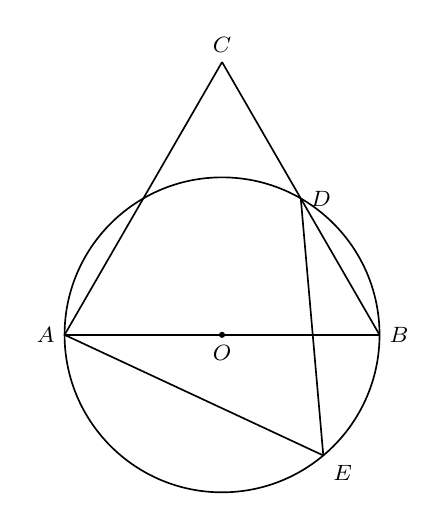
\begin{tikzpicture}[x=1cm, y=1cm, line width=0.6pt, font=\footnotesize]

  \coordinate (O)  at (0,0);
  \coordinate (A)  at (-2,0);
  \coordinate (B)  at (2,0);
  \coordinate (D)  at (1.00,1.732);
  \coordinate (C)  at (0,3.464);
  \coordinate (E)  at (1.286,-1.532);

  % ---------- 圆与直径 ----------
  \draw (0,0) circle (2);
  \draw (A) -- (B);

  % ---------- 题设线段 ----------
  \draw (B) -- (D) -- (C);
  \draw (A) -- (C);
  \draw (A) -- (E);
  \draw (D) -- (E);

  % ---------- 点与标注 ----------
  \fill (O) circle (1.1pt);
  \node[below]       at (O) {$O$};
  \node[left]        at (A) {$A$};
  \node[right]       at (B) {$B$};
  \node[right]       at (D) {$D$};
  \node[above]       at (C) {$C$};
  \node[below right] at (E) {$E$};

\end{tikzpicture}
\end{center}
\nopagebreak[4]
（2） 【B】已知矩阵 $\boldsymbol A$ 的逆矩阵 $\boldsymbol A^{-1}=\begin{bmatrix}-\dfrac14&\dfrac34\\[4pt]\dfrac12&-\dfrac12\end{bmatrix}$，求矩阵 $\boldsymbol A$ 的特征值。

（3） 【C】在极坐标系中，已知圆 $C$ 经过点 $P\left(\sqrt2,\dfrac\pi4\right)$，圆心为直线 $\rho\sin\left(\theta-\dfrac\pi3\right)=-\dfrac{\sqrt3}{2}$ 与极轴的交点，求圆 $C$ 的极坐标方程。

（4） 【D】已知实数 $x$，$y$ 满足：$|x+y|<\dfrac13$，$|2x-y|<\dfrac16$，求证：$|y|<\dfrac{5}{18}$。

\Needspace{4\baselineskip}
\textbf{解析}

\textbf{（1）【A】几何证明选讲}

\Needspace{5\baselineskip}
因为 $AB$ 是圆 $O$ 的直径，$D$ 在圆上，由直径所对圆周角为直角得
\nopagebreak[4]
\[AD\perp BD,\quad\text{\text{即} }AD\perp BC.\]
\Needspace{5\baselineskip}
又 $BD=DC$，即 $D$ 是 $BC$ 的中点，故 $AD$ 是 $BC$ 的垂直平分线，于是
\nopagebreak[4]
\[AB=AC,\]
\Needspace{5\baselineskip}
从而 $\triangle ABC$ 为等腰三角形，
\nopagebreak[4]
\[\angle ABC=\angle ACB.\]
\Needspace{5\baselineskip}
$C$ 在 $BD$ 的延长线上，故 $\angle ABC=\angle ABD$；而 $A$，$B$，$D$，$E$ 四点共圆，$\angle ABD$ 与 $\angle AED$ 所对的是同一段弧 $AD$（$B$、$E$ 在弦 $AD$ 的同侧，都不在被截取的那段弧上），故
\nopagebreak[4]
\[\angle AED=\angle ABD.\]
\Needspace{5\baselineskip}
又 $\angle ACB$ 与 $\angle C$ 是同一个角（$D$ 在 $BC$ 上，$\angle ACD=\angle ACB$），综上
\nopagebreak[4]
\[\angle E=\angle AED=\angle ABD=\angle ABC=\angle ACB=\angle C.\]

\textbf{（2）【B】矩阵与变换}

\Needspace{5\baselineskip}
设 $\boldsymbol A=\begin{bmatrix}a&b\\c&d\end{bmatrix}$。由 $\boldsymbol A\boldsymbol A^{-1}=\boldsymbol E$：
\nopagebreak[4]
\[\begin{bmatrix}a&b\\c&d\end{bmatrix}\begin{bmatrix}-\frac14&\frac34\\[2pt]\frac12&-\frac12\end{bmatrix}=\begin{bmatrix}1&0\\0&1\end{bmatrix}.\]
\Needspace{5\baselineskip}
逐元素比较：
\nopagebreak[4]
\[-\frac a4+\frac b2=1,\qquad\frac{3a}4-\frac b2=0,\qquad-\frac c4+\frac d2=0,\qquad\frac{3c}4-\frac d2=1.\]
\Needspace{5\baselineskip}
由第二式 $b=\dfrac{3a}{2}$，代入第一式 $-\dfrac a4+\dfrac{3a}4=1$，得 $a=2$，$b=3$；由第三式 $d=\dfrac c2$，代入第四式 $\dfrac{3c}4-\dfrac c4=1$，得 $c=2$，$d=1$。故
\nopagebreak[4]
\[\boldsymbol A=\begin{bmatrix}2&3\\2&1\end{bmatrix}.\]
\Needspace{5\baselineskip}
特征多项式
\nopagebreak[4]
\[\left|\lambda\boldsymbol E-\boldsymbol A\right|=\begin{vmatrix}\lambda-2&-3\\-2&\lambda-1\end{vmatrix}=(\lambda-2)(\lambda-1)-6=\lambda^2-3\lambda-4=(\lambda-4)(\lambda+1).\]
\Needspace{5\baselineskip}
令其为零得特征值
\nopagebreak[4]
\[\lambda_1=4,\qquad\lambda_2=-1.\]
核对：$\det\boldsymbol A=2-6=-4$，而 $\lambda_1\lambda_2=-4$；$\operatorname{tr}\boldsymbol A=3=\lambda_1+\lambda_2$，与特征值的和积关系一致。

\textbf{（3）【C】坐标系与参数方程}

\Needspace{5\baselineskip}
直线 $\rho\sin\left(\theta-\dfrac\pi3\right)=-\dfrac{\sqrt3}{2}$ 与极轴（$\theta=0$）的交点满足
\nopagebreak[4]
\[\rho\sin\left(-\frac\pi3\right)=-\frac{\sqrt3}{2}\Longrightarrow-\frac{\sqrt3}{2}\rho=-\frac{\sqrt3}{2}\Longrightarrow\rho=1,\]
故圆心的极坐标为 $(1,0)$，其直角坐标也是 $(1,0)$。

\Needspace{5\baselineskip}
点 $P\left(\sqrt2,\dfrac\pi4\right)$ 的直角坐标为
\nopagebreak[4]
\[x=\sqrt2\cos\frac\pi4=1,\qquad y=\sqrt2\sin\frac\pi4=1,\]
\Needspace{5\baselineskip}
即 $P(1,1)$。于是圆的半径
\nopagebreak[4]
\[r=|OP|=\sqrt{(1-1)^2+(1-0)^2}=1.\]
\Needspace{5\baselineskip}
圆 $C$ 的直角坐标方程为
\nopagebreak[4]
\[(x-1)^2+y^2=1\Longrightarrow x^2+y^2=2x.\]
\Needspace{5\baselineskip}
代入 $x=\rho\cos\theta$，$x^2+y^2=\rho^2$：
\nopagebreak[4]
\[\rho^2=2\rho\cos\theta\Longrightarrow\rho=2\cos\theta\]
（极点 $\rho=0$ 也满足该方程）。所以圆 $C$ 的极坐标方程为 $\rho=2\cos\theta$。

\textbf{（4）【D】不等式选讲}

\Needspace{5\baselineskip}
注意到恒等变形
\nopagebreak[4]
\[3y=2(x+y)-(2x-y),\]
\Needspace{5\baselineskip}
由绝对值不等式 $|u-v|\leqslant|u|+|v|$ 得
\nopagebreak[4]
\[|3y|\leqslant2|x+y|+|2x-y|<2\times\frac13+\frac16=\frac56,\]
\Needspace{5\baselineskip}
故
\nopagebreak[4]
\[|y|<\frac{5}{18}.\]
说明：关键是把 $y$ 用已知的两个线性式表示成 $2(x+y)-(2x-y)$，使 $x$ 的系数相消而 $y$ 的系数为 $3$。

\gkanswer{答案（1）：证明见解析（$\angle E$ 指 $\angle AED$，结论为 $\angle AED=\angle C$）。}

\gkanswer{答案（2）：$\lambda_1=4$，$\lambda_2=-1$。先由 $\boldsymbol A^{-1}$ 求 $\boldsymbol A=\begin{bmatrix}2&3\\2&1\end{bmatrix}$。}

\gkanswer{答案（3）：$\rho=2\cos\theta$。圆心为 $(1,0)$，半径 $1$。}

\gkanswer{答案（4）：证明见解析（由 $3y=2(x+y)-(2x-y)$ 及绝对值不等式得 $|3y|<\dfrac56$）。}

\end{answer}
\begin{answer}
\gksolhead{22}{}

\textbf{题目}：

设 $\xi$ 为随机变量，从棱长为 $1$ 的正方体的 $12$ 条棱中任取两条，当两条棱相交时，$\xi=0$；当两条棱平行时，$\xi$ 的值为两条棱之间的距离；当两条棱异面时，$\xi=1$。

（1） 求概率 $P(\xi=0)$；

（2） 求 $\xi$ 的分布列，并求其数学期望 $E(\xi)$。

\Needspace{4\baselineskip}
\textbf{解析}

\Needspace{5\baselineskip}
正方体共 $12$ 条棱，任取两条，基本事件总数为
\nopagebreak[4]
\[\mathrm C_{12}^2=\frac{12\times11}{2}=66.\]

\textbf{（1）}

\Needspace{5\baselineskip}
相交的两条棱必共用一个顶点。每个顶点处有 $3$ 条棱，两两相交，给出 $\mathrm C_3^2=3$ 对；正方体有 $8$ 个顶点，且两条相交的棱只在一个公共顶点处相遇（不会重复计数），故相交的棱共
\nopagebreak[4]
\[8\times3=24\text{ \text{对}}.\]
\Needspace{5\baselineskip}
所以
\nopagebreak[4]
\[P(\xi=0)=\frac{24}{66}=\frac4{11}.\]

\textbf{（2）}

平行的棱按方向分为 $3$ 组，每组 $4$ 条。同一组内任取两条都平行，共 $3\times\mathrm C_4^2=18$ 对。固定一个方向，这 $4$ 条棱位于与方向垂直的截面正方形的四个顶点处，任取两条的情形为：

\begin{itemize}
\item 相邻位置（共面且在同一侧面内），距离为 $1$，每个方向 $4$ 对，共 $12$ 对；
\item 对角位置（不在同一侧面内），距离为 $\sqrt2$，每个方向 $2$ 对，共 $6$ 对。
\end{itemize}

\Needspace{5\baselineskip}
既不相交也不平行的两条棱为异面直线，共
\nopagebreak[4]
\[66-24-18=24\text{ \text{对}}.\]
\Needspace{5\baselineskip}
于是
\nopagebreak[4]
\[P(\xi=1)=P(\text{\text{异面}})+P(\text{\text{平行且距离为} }1)=\frac{24}{66}+\frac{12}{66}=\frac{36}{66}=\frac6{11},\]
\nopagebreak[4]
\[P\left(\xi=\sqrt2\right)=\frac{6}{66}=\frac1{11}.\]
分布列为

\begin{center}
\begin{tabular}{llll}
\toprule
$\xi$ & $0$ & $1$ & $\sqrt2$ \\
\midrule
$P$ & $\dfrac4{11}$ & $\dfrac6{11}$ & $\dfrac1{11}$ \\
\bottomrule
\end{tabular}
\end{center}

\Needspace{5\baselineskip}
数学期望
\nopagebreak[4]
\[E(\xi)=0\times\frac4{11}+1\times\frac6{11}+\sqrt2\times\frac1{11}=\frac{6+\sqrt2}{11}.\]
核对：$\dfrac4{11}+\dfrac6{11}+\dfrac1{11}=1$，且 $0<E(\xi)=\dfrac{7.414}{11}\approx0.674<\sqrt2$，合理。

\gkanswer{答案（1）：$\dfrac4{11}$。相交的棱共 $24$ 对，总对数为 $\mathrm C_{12}^2=66$。}

\gkanswer{答案（2）：分布列为 $P(\xi=0)=\dfrac4{11}$，$P(\xi=1)=\dfrac6{11}$，$P(\xi=\sqrt2)=\dfrac1{11}$；$E(\xi)=\dfrac{6+\sqrt2}{11}$。}

\end{answer}
\begin{answer}
\gksolhead{23}{}

\textbf{题目}：

设集合 $P_n=\{1,2,\cdots,n\}$，$n\in\mathbf N^*$。记 $f(n)$ 为同时满足下列条件的集合 $A$ 的个数：① $A\subseteq P_n$；② 若 $x\in A$，则 $2x\notin A$；③ 若 $x\in\complement_{P_n}A$，则 $2x\notin\complement_{P_n}A$。

（1） 求 $f(4)$；

（2） 求 $f(n)$ 的解析式（用 $n$ 表示）。

\Needspace{4\baselineskip}
\textbf{解析}

\Needspace{5\baselineskip}
条件②③合起来即：对每个满足 $2x\leqslant n$ 的正整数 $x$，
\nopagebreak[4]
\[x\in A\Longleftrightarrow2x\notin A,\]
也就是 $x$ 与 $2x$ 中恰有一个属于 $A$。

\Needspace{5\baselineskip}
把 $1,2,\cdots,n$ 按“去掉全部因子 $2$”后的奇数分类，得到若干条链
\nopagebreak[4]
\[C_o=\left\{o,\,2o,\,4o,\,\cdots\right\}\cap\{1,2,\cdots,n\}\qquad(o\text{ \text{为奇数}},\ o\leqslant n).\]
同一链内相邻两项恰是 $(x,2x)$ 的关系，故链内元素的归属由第一项 $o$ 决定并交替排列；不同链之间没有任何约束。因此每个奇数 $o\leqslant n$ 都贡献一个二选一的自由度。

\textbf{（1）}

\Needspace{5\baselineskip}
$n=4$ 时，奇数 $o$ 为 $1,3$，两条链分别是
\nopagebreak[4]
\[C_1=\{1,2,4\},\qquad C_3=\{3\}.\]
\Needspace{5\baselineskip}
$C_1$ 中须 $1$ 与 $2$ 一取一舍、$2$ 与 $4$ 一取一舍，故 $A\cap C_1$ 只能是 $\{1,4\}$ 或 $\{2\}$；$C_3$ 中 $3$ 可任意取舍。共
\nopagebreak[4]
\[2\times2=4\]
\Needspace{5\baselineskip}
个集合，即
\nopagebreak[4]
\[\{2\},\quad\{2,3\},\quad\{1,4\},\quad\{1,3,4\}.\]
\Needspace{5\baselineskip}
直接验证 $\{1,4\}$：$1\in A$ 而 $2\notin A$，$2\notin A$ 而 $4\in A$，满足②③；其余三个同理。所以
\nopagebreak[4]
\[f(4)=4.\]

\textbf{（2）}

\Needspace{5\baselineskip}
$1,2,\cdots,n$ 中奇数的个数为 $\left\lceil\dfrac n2\right\rceil$，每个奇数确定一条链并贡献 $2$ 种选择，故
\nopagebreak[4]
\[f(n)=2^{\left\lceil\frac n2\right\rceil},\]
\Needspace{5\baselineskip}
即
\nopagebreak[4]
\[f(n)=\begin{cases}2^{\frac n2},&n\text{ \text{为偶数}},\\[4pt]2^{\frac{n+1}{2}},&n\text{ \text{为奇数}}.\end{cases}\]
核对：$n=1$ 时 $f(1)=2$（$\varnothing$ 与 $\{1\}$）；$n=2$ 时链为 $\{1,2\}$，$f(2)=2$；$n=3$ 时 $f(3)=2^2=4$；$n=4$ 时 $f(4)=2^2=4$，与（1）一致。

\gkanswer{答案（1）：$4$。满足条件的集合为 $\{2\}$，$\{2,3\}$，$\{1,4\}$，$\{1,3,4\}$。}

\gkanswer{答案（2）：$f(n)=2^{\lceil n/2\rceil}$，即 $n$ 为偶数时 $f(n)=2^{n/2}$，$n$ 为奇数时 $f(n)=2^{(n+1)/2}$。}

\end{answer}